% Options for packages loaded elsewhere
\PassOptionsToPackage{unicode}{hyperref}
\PassOptionsToPackage{hyphens}{url}
\PassOptionsToPackage{dvipsnames,svgnames,x11names}{xcolor}
%
\documentclass[
    behavsci,
    article,
    submit,
moreauthors
]{mdpi}


\usepackage{amsmath,amssymb}
\usepackage{iftex}
\ifPDFTeX
  \usepackage[T1]{fontenc}
  \usepackage[utf8]{inputenc}
  \usepackage{textcomp} % provide euro and other symbols
\else % if luatex or xetex
  \usepackage{unicode-math}
  \defaultfontfeatures{Scale=MatchLowercase}
  \defaultfontfeatures[\rmfamily]{Ligatures=TeX,Scale=1}
\fi
\usepackage{lmodern}
\ifPDFTeX\else  
    % xetex/luatex font selection
\fi
% Use upquote if available, for straight quotes in verbatim environments
\IfFileExists{upquote.sty}{\usepackage{upquote}}{}
\IfFileExists{microtype.sty}{% use microtype if available
  \usepackage[]{microtype}
  \UseMicrotypeSet[protrusion]{basicmath} % disable protrusion for tt fonts
}{}
\makeatletter
\@ifundefined{KOMAClassName}{% if non-KOMA class
  \IfFileExists{parskip.sty}{%
    \usepackage{parskip}
  }{% else
    \setlength{\parindent}{0pt}
    \setlength{\parskip}{6pt plus 2pt minus 1pt}}
}{% if KOMA class
  \KOMAoptions{parskip=half}}
\makeatother
\usepackage{xcolor}
\setlength{\emergencystretch}{3em} % prevent overfull lines
\setcounter{secnumdepth}{-\maxdimen} % remove section numbering
% Make \paragraph and \subparagraph free-standing
\makeatletter
\ifx\paragraph\undefined\else
  \let\oldparagraph\paragraph
  \renewcommand{\paragraph}{
    \@ifstar
      \xxxParagraphStar
      \xxxParagraphNoStar
  }
  \newcommand{\xxxParagraphStar}[1]{\oldparagraph*{#1}\mbox{}}
  \newcommand{\xxxParagraphNoStar}[1]{\oldparagraph{#1}\mbox{}}
\fi
\ifx\subparagraph\undefined\else
  \let\oldsubparagraph\subparagraph
  \renewcommand{\subparagraph}{
    \@ifstar
      \xxxSubParagraphStar
      \xxxSubParagraphNoStar
  }
  \newcommand{\xxxSubParagraphStar}[1]{\oldsubparagraph*{#1}\mbox{}}
  \newcommand{\xxxSubParagraphNoStar}[1]{\oldsubparagraph{#1}\mbox{}}
\fi
\makeatother


\providecommand{\tightlist}{%
  \setlength{\itemsep}{0pt}\setlength{\parskip}{0pt}}\usepackage{longtable,booktabs,array}
\usepackage{calc} % for calculating minipage widths
% Correct order of tables after \paragraph or \subparagraph
\usepackage{etoolbox}
\makeatletter
\patchcmd\longtable{\par}{\if@noskipsec\mbox{}\fi\par}{}{}
\makeatother
% Allow footnotes in longtable head/foot
\IfFileExists{footnotehyper.sty}{\usepackage{footnotehyper}}{\usepackage{footnote}}
\makesavenoteenv{longtable}
\usepackage{graphicx}
\makeatletter
\def\maxwidth{\ifdim\Gin@nat@width>\linewidth\linewidth\else\Gin@nat@width\fi}
\def\maxheight{\ifdim\Gin@nat@height>\textheight\textheight\else\Gin@nat@height\fi}
\makeatother
% Scale images if necessary, so that they will not overflow the page
% margins by default, and it is still possible to overwrite the defaults
% using explicit options in \includegraphics[width, height, ...]{}
\setkeys{Gin}{width=\maxwidth,height=\maxheight,keepaspectratio}
% Set default figure placement to htbp
\makeatletter
\def\fps@figure{htbp}
\makeatother

% TODO: Add custom LaTeX header directives here
\usepackage{booktabs}
\usepackage{longtable}
\usepackage{array}
\usepackage{multirow}
\usepackage{wrapfig}
\usepackage{float}
\usepackage{colortbl}
\usepackage{pdflscape}
\usepackage{tabu}
\usepackage{threeparttable}
\usepackage{threeparttablex}
\usepackage[normalem]{ulem}
\usepackage{makecell}
\usepackage{xcolor}
\usepackage{threeparttable}
\usepackage{graphicx}

\includegraphics{pics/logo-mdpi.pdf}
\makeatletter
\@ifpackageloaded{caption}{}{\usepackage{caption}}
\AtBeginDocument{%
\ifdefined\contentsname
  \renewcommand*\contentsname{Table of contents}
\else
  \newcommand\contentsname{Table of contents}
\fi
\ifdefined\listfigurename
  \renewcommand*\listfigurename{List of Figures}
\else
  \newcommand\listfigurename{List of Figures}
\fi
\ifdefined\listtablename
  \renewcommand*\listtablename{List of Tables}
\else
  \newcommand\listtablename{List of Tables}
\fi
\ifdefined\figurename
  \renewcommand*\figurename{Figure}
\else
  \newcommand\figurename{Figure}
\fi
\ifdefined\tablename
  \renewcommand*\tablename{Table}
\else
  \newcommand\tablename{Table}
\fi
}
\@ifpackageloaded{float}{}{\usepackage{float}}
\floatstyle{ruled}
\@ifundefined{c@chapter}{\newfloat{codelisting}{h}{lop}}{\newfloat{codelisting}{h}{lop}[chapter]}
\floatname{codelisting}{Listing}
\newcommand*\listoflistings{\listof{codelisting}{List of Listings}}
\makeatother
\makeatletter
\makeatother
\makeatletter
\@ifpackageloaded{caption}{}{\usepackage{caption}}
\@ifpackageloaded{subcaption}{}{\usepackage{subcaption}}
\makeatother
\ifLuaTeX
  \usepackage{selnolig}  % disable illegal ligatures
\fi
\usepackage[]{natbib}
\bibliographystyle{plainnat}
\usepackage{bookmark}

\IfFileExists{xurl.sty}{\usepackage{xurl}}{} % add URL line breaks if available
\urlstyle{same} % disable monospaced font for URLs
\hypersetup{
  pdftitle={The socialization of meritocracy and market justice preferences at school},
  pdfauthor={Equipo EDUMER},
  pdfkeywords={market
justice, meritocracy, socialization, family, schools, Chile},
  pdfcreator={LaTeX via pandoc},
  unicode=true,
	bookmarksopen={true},
	pdffitwindow=true, 
	colorlinks=true, 
	linkcolor=bluecite, 
	citecolor=bluecite, 
	urlcolor=bluecite, 
	hyperfootnotes=true, 
	pdfstartview={FitH},
	pdfpagemode= UseNone}

\firstpage{1} 
\makeatletter 
\setcounter{page}{\@firstpage} 
\makeatother
\pubvolume{1}
\issuenum{1}
\articlenumber{0}
\pubyear{\the\year{}}
\copyrightyear{\the\year{}}
%\externaleditor{Academic Editor: Firstname Lastname}
\datereceived{ } 
\daterevised{ } % Comment out if no revised date
\dateaccepted{ } 
\datepublished{ } 
%\datecorrected{} % For corrected papers: "Corrected: XXX" date in the original paper.
%\dateretracted{} % For corrected papers: "Retracted: XXX" date in the original paper.
\hreflink{https://doi.org/} % If needed use \linebreak
%\doinum{}
%\pdfoutput=1 % Uncommented for upload to arXiv.org
%\CorrStatement{yes}  % For updates

\Title{ The socialization of meritocracy and market justice preferences
at school }

% MDPI internal command: Title for citation in the left column
\TitleCitation{ The socialization of meritocracy and market justice
preferences at school }



% Author Orchid ID: enter ID or remove command
%\newcommand{\orcidauthorA}{0000-0000-0000-000X} % Add \orcidA{} behind the author's name
%\newcommand{\orcidauthorB}{0000-0000-0000-000X} % Add \orcidB{} behind the author's name


% Authors, for the paper (add full first names)
%\Author{Firstname Lastname $^{1,\dagger,\ddagger}$\orcidA{}, Firstname Lastname $^{2,\ddagger}$ and Firstname Lastname $^{2,}$*}

\Author{Juan Carlos Castillo$^{aff-1}$, 
Mauricio Salgado$^{aff-2}$, 
Kevin Carrasco$^{aff-3}$~and~Andreas Laffert$^{aff-4}$
}
%\longauthorlist{yes}

% MDPI internal command: Authors, for metadata in PDF
\AuthorNames{
  Juan Carlos Castillo,
  Mauricio Salgado,
  Kevin Carrasco,
  Andreas Laffert}

% MDPI internal command: Authors, for citation in the left column
%\AuthorCitation{Lastname, F.; Lastname, F.; Lastname, F.}
%\usepackage{xstring}
\newcommand\getfirst[1]{\getfirstaux#1\relax} \def\getfirstaux#1#2\relax{#1}
\newcommand{\authorformatted}{Castillo, \getfirst{Juan Carlos}.; Salgado, \getfirst{Mauricio}.; Carrasco, \getfirst{Kevin}.; Laffert, \getfirst{Andreas}.}
\AuthorCitation{\authorformatted}

% If this is a Chicago style journal: Lastname, Firstname, Firstname Lastname, and Firstname Lastname.

% Affiliations / Addresses (Add [1] after \address if there is only one affiliation.)
\address {%
$^{aff-1}$ \quad , Department of Sociology, Universidad de Chile\\
$^{aff-2}$ \quad , Centro de Estudios Públicos, Chile\\
$^{aff-3}$ \quad , Center for Social Conflict and Cohesion Studies\\
$^{aff-4}$ \quad , Institute of Sociology, Universidad Católica de
Chile\\
}

%\address{
%$^{1}$ \quad Affiliation 1; e-mail@e-mail.com\\
%$^{2}$ \quad Affiliation 2; e-mail@e-mail.com}

% Contact information of the corresponding author
%% see: https://quarto.org/docs/journals/authors.html
\corres{Correspondence: juancastillov@uchile.cl}

% Current address and/or shared authorship
%\firstnote{Current address: Affiliation.}  % Current address should not be the same as any items in the Affiliation section.
%\secondnote{These authors contributed equally to this work.}
% The commands \thirdnote{} till \eighthnote{} are available for further notes

%\simplesumm{} % Simple summary

%\conference{} % An extended version of a conference paper

% Abstract (Do not insert blank lines, i.e. \\) 
\abstract{ Previous research has shown that schools justify student
performance differences based on meritocratic ideals. However, the link
between school meritocracy and students' justification of inequalities
has received little attention. This paper examines how school and family
socialization influence students' beliefs about meritocracy and
market-based justifications for access to health, pensions, and
education in Chile. Using data from the First Study of Civic Education
in Chile, we employ a multilevel modeling strategy to analyze 5,047
students and parents nested within 231 schools. Our findings reveal that
a significant proportion of Chilean students agree with market justice
principles, at a higher rate than adults. Most students endorse
meritocratic views, particularly the reward of effort. Multilevel
estimations show strong associations between meritocratic beliefs and
market justice preferences: students who believe in the reward of effort
and talent are more likely to justify inequalities based on financial
capacity. At the school level, market justice preferences are higher in
high-status schools but lower in schools with better achievement.
Additionally, the conditional influence of meritocracy beliefs weakens
in schools with higher socioeconomic status and performance. These
results suggest that meritocratic beliefs and market justice preferences
begin early and are influenced by the school environment. }

% Keywords
\keyword{market
justice; meritocracy; socialization; family; schools; Chile}

\begin{document}

\section{Introduction}\label{introduction}

Since its origins, educational institutions have been related to the
idea of social mobility and access to better opportunities. Despite
this, the consistent evidence of the high level of social reproduction
at the school level represents a threat to the promise of education and
a meritocratic system \citep{bourdieu_reproduction_1990}. A large part
of the research in this field at an international level has addressed
the extent to which the social origin of students affects their academic
results and their life opportunities \citep{vonhippel_test_2019},
confirming that schools have severe difficulties in closing the
socio-economic and cultural gaps of origin. Besides this socioeconomic
perspective on school opportunities, recent research has addressed to
what extent inequalities in the school context are also influencing
students' perceptions, beliefs, and attitudes: Are social inequalities
even perceived at the school context? Are they rejected by the students,
particularly those who are worst-off in socioeconomic terms? Or, Is
there evidence at the school level that social inequalities are
tolerated and even justified?
\citep{batruch_belief_2022, wiederkehr_belief_2015}.

Given that the school environment has an important focus on performance,
achievement and acknowledgment, meritocracy has been one of the
principal concepts used for understanding and even for justifying
performance differences among students. Meritocracy is a distributive
system based on the belief that people should be rewarded and promoted
based on their abilities, knowledge, and achievements
\citep{young_rise_1958}. It is often seen as a way to create equal
opportunities and fairness, as individuals can rise to positions of
power and influence based on their own merit rather than their
background or connections. However, some argue that meritocracy can
actually lead to tolerating or even justifying social inequalities, as
it can create a hierarchy where those who already have resources and
advantages are more likely to succeed
\citep{sandel_tyranny_2020, mcnamee_meritocracy_2004}. In this regard, a
great deal of academic research about meritocracy delves into the
assessment of to what extent rewards and privileges in society are
related to merit, emphasizing the so-called unfulfillable promise of
meritocracy \citep{mijs_stratified_2016}.

In the present paper, we address the role of the perception of
meritocracy on the justification of social inequalities by eighth-grade
students in Chile, a country characterized by a highly stratified
educational system. In particular, we focus on justifying inequalities
in health, education and pensions, which are traditional social policy
areas where access to better services could be justified based on
payment capacity, referred to as market justice
\citep{lane_market_1986, lindh_bringing_2023}. Most of the research in
this realm has only considered adults, leaving aside the study of how
beliefs in this field develop at student age as well as the impact of
the school context and the family as the main socialization agencies
\citep{batruch_belief_2022}. Regarding schools, the way in which they
deal with unequal conditions of origin has been linked to the
\emph{hidden curriculum} \citep{chafel_schooling_1997}, whereby students
learn about distributive norms in society and mechanisms of
justification of social differences.

Based on recent studies that relate school meritocracy to the
justification of economic inequalities in the adult population
\citep{batruch_belief_2022, wiederkehr_belief_2015}, the central
hypothesis guiding this research is that school-age students with a
higher perception of meritocracy - both at school and at the societal
level - will show a larger market justice preferences, as individual
achievement would be seen as appropriately rewarded and social
mechanisms for correcting inequalities as less necessary
\citep{batruch_belief_2022}. We focus on the student-age population as
we point out that it is possible to track down the origin of
meritocratic beliefs (and their consequences) to early socialization
processes. To this regard, we take into account the family and the
school as two main socialization agencies that play a significant role
in the socialization of cultural beliefs by transmitting cultural norms,
values, and expectations to young people.

The Chilean case is particularly intriguing for studying market justice
preferences. This country is characterized by acute and persistent
economic inequality, which stands out in Latin America and among OECD
countries \citep{flores_top_2020}. In Chile, the poorest 50\% captures
only 10\% of the total income and has negative wealth, while the richest
1\% receives almost 27\% of the income and holds 49.6\% of the wealth
\citep{chancel_world_2022}. Much of this inequality has been attributed
to the deep neoliberal reforms that institutionalized privatization and
commodification of various economic sectors. Such reforms where
introduced during the dictatorship (1973-1989) and expanded in democracy
through concessions, demand credits, and specific regulatory frameworks
\citep{ffrench-davis_reformas_2018}. This shift in economic policy has
allowed the unprecedented emergence of markets in areas related to
social reproduction, such as health, pensions, and education, with
provision and access managed by private entities and segmented by
individual payment capacity, heavily reliant on State subsidies
\citep{boccardo_30_2020}. In health, although the majority of the
population uses the public insurance system (78.9\%), 15.3\% are served
by private insurers \citep{observatoriosocial_estadisticas_2024}. The
pension system is based on individual capitalization, with mandatory
contributions managed by private administrators investing in the
financial market, currently involving 11 million contributors
\citep{superintendenciadepensiones_estadisticas_2024}. In education,
30.6\% of school enrollment is in public schools, 54.0\% in
state-subsidized (voucher) private schools, and 9.3\% in fully private
schools, generally attracting higher-income groups
\citep{ministeriodeeducacion_resumen_2023}.

\subsection{Justification of inequality and market
justice}\label{justification-of-inequality-and-market-justice}

The justification of social inequality based on market-type criteria has
been conceptualized as the individuals' adherence to the deservingness
of social goods and services (such as health, education, and pensions)
based on prices and individuals' ability to pay
\citep{boltanski_new_2005, lane_market_1986, streeck_citizens_2012}.
Research on social stratification beliefs, which explore individual
perceptions of who deserves what and why \citep{kluegel_beliefs_1987},
highlights that people's explanations and justifications of social
inequality are closely tied to their judgments of deservingness. The
influence of ideologies \citep{wegener_dominant_1995} and cultural
schemas \citep{homan_being_2017} is pivotal in shaping these
explanations by offering symbolic representations that frame societal
structures and expectations. While significant attention has been paid
to wage inequality, income distribution, and payment differentials in
the literature
\citep{castillo_legitimacy_2011, evans_family_2010, jasso_how_1999, shariff_income_2016},
there has been less examination of public beliefs about which life
domains should be governed by market relations
\citep{lindh_bringing_2023} and even less about children's acceptance or
rejection of these market principles. This oversight is notable given
the extensive encroachment of market logic into public goods, welfare
policy, and social services over the past five decades
\citep{centeno_arc_2012, harvey_breve_2015}, affecting areas such as
pensions, health services, and education.

There are substantial differences in funding and delivery methods in the
management of social services across nations
\citep{jensen_worlds_2008, stoy_worlds_2014}. Nordic countries, for
example, predominantly employ public agencies to produce and provide
social services, funding these through collective taxation and offering
them in kind to the majority of citizens. This system prioritizes social
justice, placing it above market mechanisms in accessing services. In
contrast, other countries rely more heavily on for-profit entities and
private funding, where service distribution depends mainly on individual
financial capacity to pay user fees, highlighting the influence of
market justice in service allocation. The trend toward marketization of
welfare services has been growing since the 1980s
\citep{salamon_marketization_1993}, and this shift is increasingly
evident even in countries where market solutions have traditionally had
a minor role in social policy \citep{sivesind_changing_2017}. The
expansion of marketization has been related to a larger justification of
market mechanisms, whereby societies with larger private spending on
services show larger market justice preferences
\citep{lindh_public_2015}.

Robert E. Lane proposed the underpinnings of the concept of market
justice, which he differentiated from political justice. For him, ``it
is the genius of the market to stimulate wants without at the same time
stimulating a sense of deserving more than one gets''
\citeyearpar[p.~384]{lane_market_1986}. Contrary to the evidence that
unequal distribution produces feelings of dissatisfaction, anger, and
resentment that might motivate forms of collective action
\citep{greitemeyer_subjective_2016, mishra_subjective_2015, smith_relative_2012, power_deprivationprotest_2018},
Lane pointed out that in market settings, social comparisons are more
likely to motivate increased effort rather than feelings of acute
injustice because individuals attribute outcomes to their actions. In
this sense, unequal levels of well-being would be, to some extent, a
function of their talents and efforts, instead of being based on
distributive principles that characterize welfare states, such as need
and equality (see \citep{wilson_role_2003}).

Despite high-income inequality and limited social mobility in Chile, and
in Latin America in general, there is a prevalent belief that
individuals are solely responsible for their economic outcomes, a view
that varies across the region
\citep{bucca_merit_2016, chong_mystery_2008, torche_intergenerational_2014, salgado_inequality_2023}.
The reliance on private welfare providers and widespread user fees
\citep{molyneux_neoliberal_2008} adds complexity to this context, as
reflected in surveys conducted by the Center for Public Studies (CEP).
According to this data, 35.9\% prefer private health insurance, and 63\%
would prefer private education
\citep{centrodeestudiospublicos_estudio_2024}. Yet, research on
children's justification in this area remains limited, highlighting a
significant gap in understanding how younger generations view
market-based access to welfare and whether these views are associated
with their meritocratic beliefs.

\subsection{Meritocratic perceptions and market
justice}\label{meritocratic-perceptions-and-market-justice}

The original definition of merit is a combination of effort and talent
\citep{young_rise_1958}, and a meritocracy is a distributive system
where merit is the main criterion for allocating valuable goods and
rewards. From a sociological perspective, meritocracy has been used in
research on social mobility to characterize societies with low mobility
that threaten the meritocratic ideal \citep{goldthorpe_myth_2003}. More
recently, sociology and social psychology research has attended to
subjective aspects related to the support for meritocratic principles in
different societies, such as beliefs in meritocracy
\citep{castillo_multidimensional_2023, mijs_unfulfillable_2016, mijs_paradox_2019}.

Meritocratic beliefs can cover two types of subjective processes:
preferences and perceptions \citep{castillo_multidimensional_2023}.
While meritocratic preferences refer to a justification of distribution
based on merit criteria (effort and talent), the perception of
meritocracy refers to how individuals view and understand the concept of
meritocracy in their society
\citep{duru-bellat_who_2012, castillo_meritocracia_2019}. The perception
can vary greatly depending on individual experiences, as well as social,
economic, and cultural background. Some people may see meritocracy as a
fair and just system that allows anyone to succeed based on their
abilities and hard work. In contrast, others may view it as a myth or a
cover for existing power dynamics and inequality, serving to maintain
and even reinforce inequality
\citep{lampert_meritocratic_2013, mijs_paradox_2019}. Some studies have
analyzed how those with greater privileges believe more in meritocracy
\citep{reynolds_perceptions_2014}, how greater economic inequality
increases meritocratic beliefs \citep{mijs_paradox_2019}, and how larger
inequality decreases it \citep{morris_representing_2022}.

A larger justification of meritocratic distribution has been related to
less support for redistributive compensation systems
\citep{frank_performance_2015}, as individual achievement would be seen
as rewarded and social policies as less necessary.
\citet{almas_cutthroat_2020} found that in the US the highly educated
accept inequality significantly more than the less educated because they
perceive inequality as justifiable owing to differences in productivity
(i.e., merit). \citet{barr_effect_2020} found that in unequal societies,
the highly educated accept inequality more than the low educated.
Conversely, individuals tend to support redistribution when they believe
that the disadvantaged lack the opportunities to succeed
\citep{evans_strong_2018}.

Schools contribute to institutionalizing and reproducing inequality by
promoting values, norms, practices, and languages familiar to
higher-class families because the dominant group's culture shapes
educational institutions \citep{bourdieu_reproduction_1990}. Middle- and
upper-class students are better equipped to face academic challenges and
are more familiar with academic expectations
\citep{mikus_children_2019}. Such familiarity represents cultural
capital in educational contexts because higher-status students come to
school ready to meet these expectations and reap the benefits
\citep{jack_no_2016, khan_privilege_2011}. Conversely, lower-status
children lacking cultural capital must catch up while experiencing
inequitable comparisons \citep{goudeau_hidden_2017}. Additionally,
academic achievement is treated as the outcome of dispositional factors
(e.g., pupils' efforts and talents or lack of them) rather than the
result of differential access to critical resources. Due to the
meritocratic frame schools encourage, both low- and high-status
individuals tend to believe that success or failure is not due to the
family background but rather to differences in efforts and talents
\citep{darnon_where_2018}. In this sense, we believe that the perception
of meritocracy can influence students' judgments about market justice
preferences, leading to our first hypothesis:

\(H_{1a}\): Students who perceive that there is more meritocracy in
society will show larger market justice preferences

The perception of meritocracy has been mostly studied with general
questions about reward allocation based on effort and talent (usually
intelligence). Nevertheless, when looking at the school population it is
possible to further consider the perception of meritocracy referred
specifically to the school context. For instance,
\citet{resh_sense_2010} find that perception of justice in grades has a
positive effect on liberal democratic orientation, and trust in people
and formal institutions \citep{resh_sense_2014}. Attending to this
evidence, we differentiate in this study between meritocratic perception
in society at large, and meritocratic perception at school, proposing
the next hypothesis:

\(H_{1b}\): Students who perceive that there is more meritocracy at
school will show larger market justice preferences

\subsection{The socialization of market justice: families and
schools}\label{the-socialization-of-market-justice-families-and-schools}

Attending to the socialization within the family, the classic work of
Kohn showed that middle-class parents value the expression of internal
states and emotions, such as self-control, curiosity, happiness, and
consideration, while working-class parents promote deference, obedience,
and conformity to authority \citep{kohn_social_1963, kohn_class_1969}.
Although parents from all social backgrounds encourage individualism in
their children, this shared norm translates into different forms in high
and low social classes \citeyearpar{kohn_class_1969}.
\citet{acemoglu_obedience_2021} claimed that the values families impart
to their children interact with social mobility. On the one hand,
children from privileged families are socialized to adopt a clear
conception of individualism that highlights their internal states,
independence, and idiosyncrasies. In contrast, children from
disadvantaged families are socialized to support a more balanced view of
individualism that considers personal characteristics as resources to
overcome collective impediments on the path to upward mobility
\citep{iacoviello_collectivism_2019}. In the same line,
\citet{almas_fairness_2017} found that adolescents from
low-socioeconomic-status families are likelier to have an egalitarian
fairness view and consider an equal distribution as fair in a situation
with unequal merits. Taking this into account, we believe that there
will be differences in the socialization of values according to
socioeconomic differences in families that could influence market
justice preferences, which leads us to the following hypothesis:

\(H_2\): Students from families of higher social status will show larger
market justice preferences.

Recent empirical research has demonstrated that the institutional design
of schools, coupled with the meritocratic ideology it fosters,
significantly influences children's and adolescents' views on inequality
and deservingness. For example, \citet{jonsson_institutional_2015} study
revealed that higher-status adolescents in Sweden tend to perpetuate
social class stereotypes while describing the vocational and academic
tracks. Academic track students are depicted as wealthy, intelligent,
ambitious, and diligent, while vocational track students are
characterized as poor, unambitious, unintelligent, and lackadaisical.
These stereotypes help individuals maintain a sense of superiority over
others and legitimize the prevailing social hierarchies and economic
disparities \citep{jost_attitudinal_2000}. In this line, and besides
status, we also expect that schools that exhibit average better
performance scores in standardized large-scale assessments would also
show larger market justice preferences. The correspondent hypotheses
are:

\(H_3\): Students from schools of higher social status will show larger
market justice preferences.

\(H_4\): Students from schools with an average better performance in
standardized achievement tests will show larger market justice
preferences.

The last set of hypotheses deals with the moderation effects. We propose
that the link between meritocracy and market justice could be stronger
for those of high status and attending schools with larger achievement
scores. In this regard, the effects of status and merit would not be
independent, as it would be expected that those who succeed in terms of
educational rewards and career paths - usually those of higher status -
perceive more meritocracy, which would reflect on larger market justice
preferences. In similar terms, schools of better performance would
promote meritocratic perception, strengthening market justice
preferences:

\(H_5\): The family's social status will moderate the effect of
meritocratic perception on market justice preferences.

\(H_6\): The school's status will moderate the effect of meritocratic
perceptions on market justice preferences.

\(H_7\): The school's performance in standardized achievement tests will
moderate the effect of meritocratic perceptions on market justice
preferences.

Figure~\ref{fig-hypotheses} depicts a summary of the research hypothesis
described before. Market justice preferences are our main concept under
study (vis-a-vis dependent variable), which refers to the justification
of better access to health, education, and pensions based on payment
capacities (as we detail further in the methods section). The
explanatory concepts (independent variables) are at two levels: student
(individual) variables and school (context) variables. The moderation
hypotheses are represented through arrows pointing to the arrow between
meritocratic perception and market justice preferences, which will be
estimated through interaction effects.

\begin{figure}

\centering{

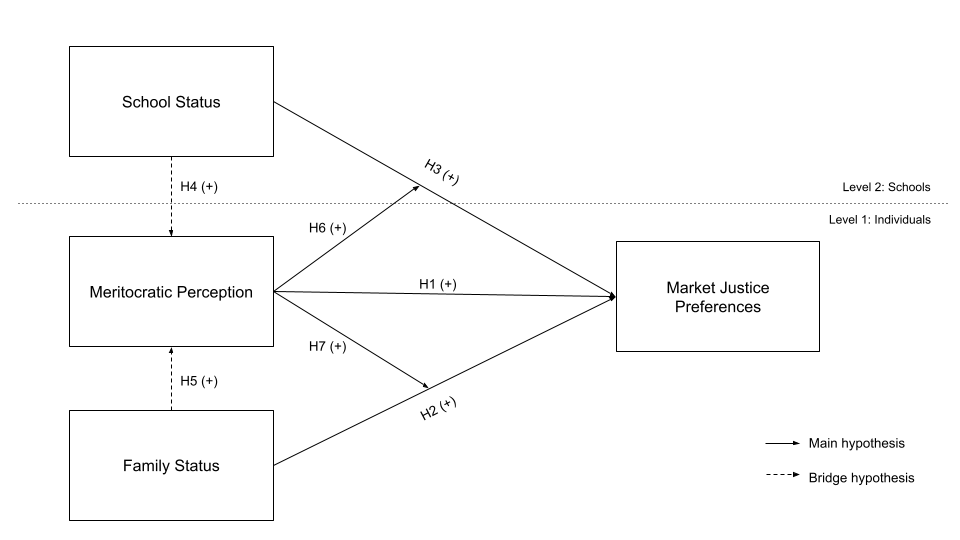
\includegraphics[width=6.25in,height=\textheight]{input/img/hypothesis2.png}

}

\caption{\label{fig-hypotheses}Summary of hypotheses}

\end{figure}%

\section{Data, variables and method}\label{data-variables-and-method}

\subsection{Data}\label{data}

The First Study of Civic Education in Chile, conducted by the Agency for
Quality Education of the Ministry of Education in 2017, serves as the
main data source. This database is composed by a civic knowledge test
score and a series of items batteries measuring different aspects of
citizenship. The target population includes 8th-grade students in 242
schools nationwide, as well as their parents and teachers. Initially,
the database contains 8,589 student observations and 6,770 parent
observations. To ensure higher data quality and considering the survey's
unit of analysis, we removed 171 student cases and 79 parent cases that
exhibited repetitive and careless response patterns
\citep{gottfried_autocorrelation_2022}. Additionally, we utilized data
from the System for Measuring the Quality of Education (SIMCE) conducted
by the Ministry of Education in 2017, which provides school-level
information such as administrative dependence, socioeconomic
classification, and results obtained in standardized mathematics and
language tests. After processing the variables and removing missing
cases, the final database for this study includes a two-level stratified
sample composed of 5,047 students and parents (level 1) nested within
231 schools (level 2).

\subsection{Variables}\label{variables}

\textbf{\emph{Individual level}}

\textbf{Market Justice Preferences}: The dependent variables in this
study are market justice preferences. This construct is measured through
three variables that address the degree of justification regarding
whether access to social services in pensions, education, and health
should be income conditional. Justification of inequality in health is
measured by the item: ``Is it fair in Chile that people with higher
incomes can access better healthcare than those with lower incomes?''
The same question is asked for education and pensions. In all cases,
respondents indicate their preferences on a Likert scale ranging from
``completely disagree'' (1) to ``completely agree'' (4). Additionally,
we include a summarized indicator of ``market justice preferences'',
measured by an average index across these items (α = 0.86), with values
ranging from 1 to 4, where higher values represent greater preferences
for market justice (see Table~\ref{tbl-desc-dependientes}). We analyzed
these items independently as well as by the average index.

\begin{longtable}[]{@{}
  >{\raggedright\arraybackslash}p{(\columnwidth - 6\tabcolsep) * \real{0.4286}}
  >{\raggedright\arraybackslash}p{(\columnwidth - 6\tabcolsep) * \real{0.2551}}
  >{\raggedright\arraybackslash}p{(\columnwidth - 6\tabcolsep) * \real{0.2143}}
  >{\raggedright\arraybackslash}p{(\columnwidth - 6\tabcolsep) * \real{0.1020}}@{}}
\caption{Dependent
variables}\label{tbl-desc-dependientes}\tabularnewline
\toprule\noalign{}
\begin{minipage}[b]{\linewidth}\raggedright
Label
\end{minipage} & \begin{minipage}[b]{\linewidth}\raggedright
Stats / Values
\end{minipage} & \begin{minipage}[b]{\linewidth}\raggedright
Freqs (\% of Valid)
\end{minipage} & \begin{minipage}[b]{\linewidth}\raggedright
Valid
\end{minipage} \\
\midrule\noalign{}
\endfirsthead
\toprule\noalign{}
\begin{minipage}[b]{\linewidth}\raggedright
Label
\end{minipage} & \begin{minipage}[b]{\linewidth}\raggedright
Stats / Values
\end{minipage} & \begin{minipage}[b]{\linewidth}\raggedright
Freqs (\% of Valid)
\end{minipage} & \begin{minipage}[b]{\linewidth}\raggedright
Valid
\end{minipage} \\
\midrule\noalign{}
\endhead
\bottomrule\noalign{}
\endlastfoot
It is just that in Chile people with higher incomes can have better
pensions than people with low incomes &
\begin{minipage}[t]{\linewidth}\raggedright
1. Strongly disagree\\
2. Disagree\\
3. Agree\\
4. Strongly agree\strut
\end{minipage} & \begin{minipage}[t]{\linewidth}\raggedright
1837 (30.6\%)\\
1945 (32.4\%)\\
1622 (27.0\%)\\
608 (10.1\%)\strut
\end{minipage} & \begin{minipage}[t]{\linewidth}\raggedright
6012\\
(95.9\%)\strut
\end{minipage} \\
It is just that in Chile people who can pay have a better education for
their children & \begin{minipage}[t]{\linewidth}\raggedright
1. Strongly disagree\\
2. Disagree\\
3. Agree\\
4. Strongly agree\strut
\end{minipage} & \begin{minipage}[t]{\linewidth}\raggedright
1766 (29.7\%)\\
1732 (29.1\%)\\
1704 (28.6\%)\\
750 (12.6\%)\strut
\end{minipage} & \begin{minipage}[t]{\linewidth}\raggedright
5952\\
(94.9\%)\strut
\end{minipage} \\
It is just that in Chile people with higher incomes can access better
health services than people with low incomes &
\begin{minipage}[t]{\linewidth}\raggedright
1. Strongly disagree\\
2. Disagree\\
3. Agree\\
4. Strongly agree\strut
\end{minipage} & \begin{minipage}[t]{\linewidth}\raggedright
2254 (38.0\%)\\
1685 (28.4\%)\\
1401 (23.6\%)\\
593 (10.0\%)\strut
\end{minipage} & \begin{minipage}[t]{\linewidth}\raggedright
5933\\
(94.6\%)\strut
\end{minipage} \\
Market Justice Preferences & \begin{minipage}[t]{\linewidth}\raggedright
Mean (sd) : 2.2 (0.9)\\
min \textless{} med \textless{} max:\\
1 \textless{} 2 \textless{} 4\\
IQR (CV) : 1.7 (0.4)\strut
\end{minipage} & 13 distinct values &
\begin{minipage}[t]{\linewidth}\raggedright
6077\\
(96.9\%)\strut
\end{minipage} \\
\end{longtable}

\textbf{Perception of Meritocracy}: The main independent variable refers
to the perception of meritocracy, operationalized through five items
addressing the perception of rewards based on talent and intelligence at
both the school and societal levels. At the school level, students
respond to whether ``Intelligence is important for getting good grades''
and ``Effort is important for getting good grades''. At the societal
level, students respond to the following questions: ``In Chile, people
are rewarded for their effort'', ``In Chile, people get what they
deserve'' and ``In Chile, people are rewarded for their intelligence and
skills''. Each item was answered on a four-point Likert scale ranging
from ``completely disagree'' (1) to ``completely agree'' (4).

\textbf{Family Socioeconomic Status}: The socioeconomic status of
students' families is measured using two indicators. First, the highest
educational level attained by the parents, with categories: ``8th grade
or less,'' ``Secondary education,'' ``Technical higher education,''
``University or postgraduate,'' and ``No response.'' The inclusion of
the ``No response'' category is due to its high frequency in the data;
omitting it could obscure relevant associations. Second, the number of
books in the household is used, categorized as ``Less than 25'' and
``More than 25.''

Table~\ref{tbl-desc-independent} shows the individual level variables
used, their response categories and their frequencies.

\begin{longtable}[]{@{}
  >{\raggedright\arraybackslash}p{(\columnwidth - 6\tabcolsep) * \real{0.3925}}
  >{\raggedright\arraybackslash}p{(\columnwidth - 6\tabcolsep) * \real{0.3084}}
  >{\raggedright\arraybackslash}p{(\columnwidth - 6\tabcolsep) * \real{0.1963}}
  >{\raggedright\arraybackslash}p{(\columnwidth - 6\tabcolsep) * \real{0.1028}}@{}}
\caption{Individual level
variables}\label{tbl-desc-independent}\tabularnewline
\toprule\noalign{}
\begin{minipage}[b]{\linewidth}\raggedright
Label
\end{minipage} & \begin{minipage}[b]{\linewidth}\raggedright
Stats / Values
\end{minipage} & \begin{minipage}[b]{\linewidth}\raggedright
Freqs (\% of Valid)
\end{minipage} & \begin{minipage}[b]{\linewidth}\raggedright
Valid
\end{minipage} \\
\midrule\noalign{}
\endfirsthead
\toprule\noalign{}
\begin{minipage}[b]{\linewidth}\raggedright
Label
\end{minipage} & \begin{minipage}[b]{\linewidth}\raggedright
Stats / Values
\end{minipage} & \begin{minipage}[b]{\linewidth}\raggedright
Freqs (\% of Valid)
\end{minipage} & \begin{minipage}[b]{\linewidth}\raggedright
Valid
\end{minipage} \\
\midrule\noalign{}
\endhead
\bottomrule\noalign{}
\endlastfoot
Intelligence is important to get good grades &
\begin{minipage}[t]{\linewidth}\raggedright
1. Strongly disagree\\
2. Disagree\\
3. Agree\\
4. Strongly agree\strut
\end{minipage} & \begin{minipage}[t]{\linewidth}\raggedright
367 ( 6.1\%)\\
920 (15.3\%)\\
2970 (49.4\%)\\
1760 (29.3\%)\strut
\end{minipage} & \begin{minipage}[t]{\linewidth}\raggedright
6017\\
(95.9\%)\strut
\end{minipage} \\
Effort is important to get good grades &
\begin{minipage}[t]{\linewidth}\raggedright
1. Strongly disagree\\
2. Disagree\\
3. Agree\\
4. Strongly agree\strut
\end{minipage} & \begin{minipage}[t]{\linewidth}\raggedright
109 ( 1.8\%)\\
88 ( 1.5\%)\\
1427 (23.7\%)\\
4406 (73.1\%)\strut
\end{minipage} & \begin{minipage}[t]{\linewidth}\raggedright
6030\\
(96.1\%)\strut
\end{minipage} \\
In Chile, people are rewarded for their intelligence and skill &
\begin{minipage}[t]{\linewidth}\raggedright
1. Strongly disagree\\
2. Disagree\\
3. Agree\\
4. Strongly agree\strut
\end{minipage} & \begin{minipage}[t]{\linewidth}\raggedright
517 ( 9.0\%)\\
1568 (27.3\%)\\
2673 (46.6\%)\\
983 (17.1\%)\strut
\end{minipage} & \begin{minipage}[t]{\linewidth}\raggedright
5741\\
(91.5\%)\strut
\end{minipage} \\
In Chile, people are rewarded for their efforts &
\begin{minipage}[t]{\linewidth}\raggedright
1. Strongly disagree\\
2. Disagree\\
3. Agree\\
4. Strongly agree\strut
\end{minipage} & \begin{minipage}[t]{\linewidth}\raggedright
512 ( 8.7\%)\\
1733 (29.4\%)\\
2607 (44.2\%)\\
1050 (17.8\%)\strut
\end{minipage} & \begin{minipage}[t]{\linewidth}\raggedright
5902\\
(94.1\%)\strut
\end{minipage} \\
In Chile, people get what they deserve &
\begin{minipage}[t]{\linewidth}\raggedright
1. Strongly disagree\\
2. Disagree\\
3. Agree\\
4. Strongly agree\strut
\end{minipage} & \begin{minipage}[t]{\linewidth}\raggedright
604 (10.5\%)\\
1911 (33.1\%)\\
2388 (41.4\%)\\
871 (15.1\%)\strut
\end{minipage} & \begin{minipage}[t]{\linewidth}\raggedright
5774\\
(92.1\%)\strut
\end{minipage} \\
Parental educational level & \begin{minipage}[t]{\linewidth}\raggedright
1. 8th grade or less\\
2. Secondary Education\\
3. Higher tec. education\\
4. University or Postgraduat\\
5. Missing\strut
\end{minipage} & \begin{minipage}[t]{\linewidth}\raggedright
559 ( 8.9\%)\\
1698 (27.1\%)\\
960 (15.3\%)\\
1080 (17.2\%)\\
1975 (31.5\%)\strut
\end{minipage} & \begin{minipage}[t]{\linewidth}\raggedright
6272\\
(100.0\%)\strut
\end{minipage} \\
Number of books at home & \begin{minipage}[t]{\linewidth}\raggedright
1. Les than 25\\
2. More than 25\strut
\end{minipage} & \begin{minipage}[t]{\linewidth}\raggedright
3920 (63.2\%)\\
2281 (36.8\%)\strut
\end{minipage} & \begin{minipage}[t]{\linewidth}\raggedright
6201\\
(98.9\%)\strut
\end{minipage} \\
\end{longtable}

\textbf{\emph{Contextual level}}

This study focuses on two school-level characteristics: socioeconomic
status and academic performance. Socioeconomic status is assessed using
the Ministry of Education's classification, measured as an ordinal item
with five categories ranging from ``low'' (1) to ``high'' (5). Academic
performance is measured using the school's results in the SIMCE (System
of Measurement of Educational Quality) standardized tests, which are
administered yearly at different educational levels in areas such as
language and mathematics. These results are categorized as ``low,''
``medium,'' and ``high.'' The contextual level items used, response
categories, and their frequencies are detailed in
Table~\ref{tbl-desc-school}.

\begin{longtable}[]{@{}
  >{\raggedright\arraybackslash}p{(\columnwidth - 6\tabcolsep) * \real{0.4138}}
  >{\raggedright\arraybackslash}p{(\columnwidth - 6\tabcolsep) * \real{0.2184}}
  >{\raggedright\arraybackslash}p{(\columnwidth - 6\tabcolsep) * \real{0.2414}}
  >{\raggedright\arraybackslash}p{(\columnwidth - 6\tabcolsep) * \real{0.1264}}@{}}
\caption{School context variables}\label{tbl-desc-school}\tabularnewline
\toprule\noalign{}
\begin{minipage}[b]{\linewidth}\raggedright
Label
\end{minipage} & \begin{minipage}[b]{\linewidth}\raggedright
Stats / Values
\end{minipage} & \begin{minipage}[b]{\linewidth}\raggedright
Freqs (\% of Valid)
\end{minipage} & \begin{minipage}[b]{\linewidth}\raggedright
Valid
\end{minipage} \\
\midrule\noalign{}
\endfirsthead
\toprule\noalign{}
\begin{minipage}[b]{\linewidth}\raggedright
Label
\end{minipage} & \begin{minipage}[b]{\linewidth}\raggedright
Stats / Values
\end{minipage} & \begin{minipage}[b]{\linewidth}\raggedright
Freqs (\% of Valid)
\end{minipage} & \begin{minipage}[b]{\linewidth}\raggedright
Valid
\end{minipage} \\
\midrule\noalign{}
\endhead
\bottomrule\noalign{}
\endlastfoot
Socioeconomic level of school &
\begin{minipage}[t]{\linewidth}\raggedright
1. Low\\
2. Medium low\\
3. Medium\\
4. Medium high\\
5. High\strut
\end{minipage} & \begin{minipage}[t]{\linewidth}\raggedright
49 (21.1\%)\\
92 (39.7\%)\\
43 (18.5\%)\\
29 (12.5\%)\\
19 ( 8.2\%)\strut
\end{minipage} & \begin{minipage}[t]{\linewidth}\raggedright
232\\
(100.0\%)\strut
\end{minipage} \\
SIMCE score achievement by school &
\begin{minipage}[t]{\linewidth}\raggedright
1. Low\\
2. Medium\\
3. High\strut
\end{minipage} & \begin{minipage}[t]{\linewidth}\raggedright
108 (46.6\%)\\
69 (29.7\%)\\
55 (23.7\%)\strut
\end{minipage} & \begin{minipage}[t]{\linewidth}\raggedright
232\\
(100.0\%)\strut
\end{minipage} \\
\end{longtable}

\textbf{\emph{Controls}}

A series of control variables are included. At the individual level, an
index of access to technology is constructed based on the number of
computers, tablets, and cell phones in the household, as well as
internet connectivity. At the contextual level, we use the
administrative dependence of schools, classified as ``Public,''
``Subsidized Private,'' or ``Private,'' and the proportion of parents
with university or postgraduate education at each school.

\subsection{Methods}\label{methods}

Given the hierarchical structure of the data, with students nested
within schools, model estimation is performed within a multilevel
framework. These models are appropriate for capturing both individual
and contextual effects in a single analysis, allowing for the estimation
of fixed effects between groups and random effects that vary from one
group to another \citep{bell_fixed_2019, hox_multilevel_2010}.
Cumulative link mixed models were employed for the ordinal dependent
variables, while linear mixed-effects models were applied for the
average market justice preference index.

The hypotheses of this research were pre-registered in the Open Science
Framework platform of the Center for Open Science (OSF), the access to
the document is available at this
\href{https://doi.org/10.17605/OSF.IO/UFSDV}{link}. The statistical
analysis for this research was conducted using the \emph{lme4} package
in R version 4.1.3.

\section{Results}\label{results}

\subsection{Descriptive}\label{descriptive}

Figure~\ref{fig-marketjustice} illustrates the distribution of responses
to the three items on market justice preferences (healthcare, pensions,
and education), indicating that most respondents tend to disagree or
strongly disagree with the idea that it is just for people with higher
incomes to have access to better services in these areas. The strongest
opposition is observed in the healthcare sector, as the majority of
respondents (66.4\%) are against the idea that higher-income individuals
should have access to better healthcare services. Similarly, regarding
the concept of justice related to access to better pensions based on
income, the level of disagreement reaches 63.0\%. This decreases
significantly in the field of education, as the percentage of
respondents who disagree or strongly disagree with those with higher
incomes having access to better education decreases to 58.8\%. Only a
small proportion agree that access to healthcare should be conditional
on income (23.6\%), and a minority strongly agree (10\%), as is the case
with pensions. However, this increases in the case of education, being
the area where there is a significant proportion of respondents who
agree or strongly agree with access based on market justice (41.2\%).

\begin{figure}

\centering{

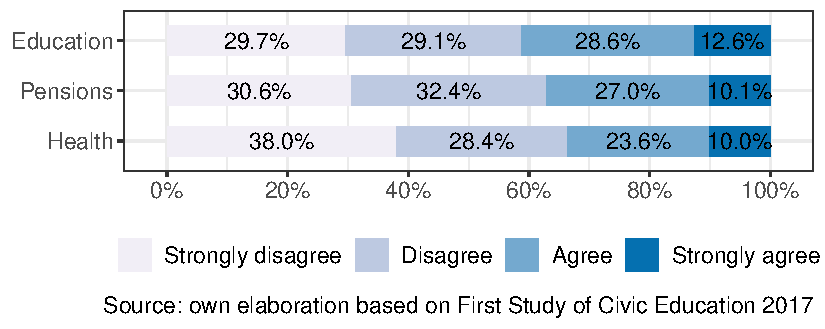
\includegraphics{paper_files/figure-pdf/fig-marketjustice-1.pdf}

}

\caption{\label{fig-marketjustice}Market justice preferences in health,
pensions and education}

\end{figure}%

Regarding the perception of meritocracy, Figure~\ref{fig-meritocracy}
displays the frequency distribution of five items related to the
dimensions of school and society. At the school level, there is a strong
belief that both effort and talent are important for achieving good
grades, with especially high agreement for effort. Specifically, while
78.6\% agree or strongly agree on the importance of talent for obtaining
good grades, this proportion rises to 96.8\% for effort, indicating that
respondents value effort more than talent in this context.

\begin{figure}

\centering{

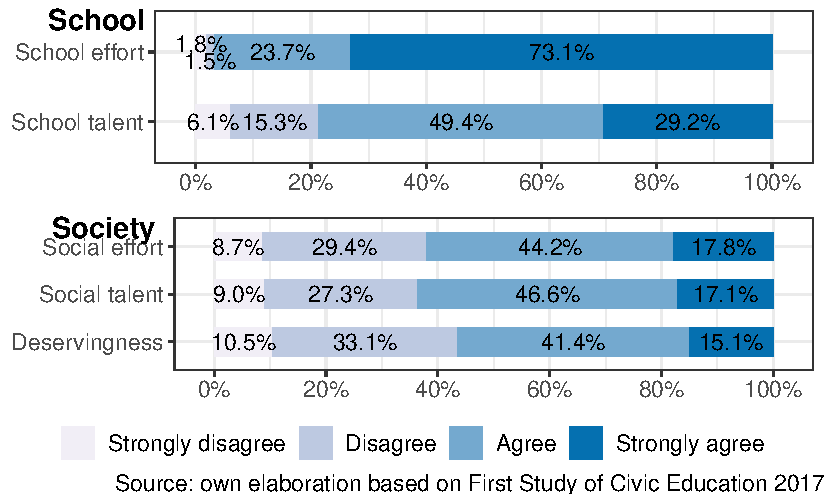
\includegraphics{paper_files/figure-pdf/fig-meritocracy-1.pdf}

}

\caption{\label{fig-meritocracy}Social and school meritocracy}

\end{figure}%

At the societal level, Figure~\ref{fig-meritocracy} shows that a
majority of respondents agree or strongly agree that individuals are
rewarded for their talents (63.7\%) and efforts (62\%). Nevertheless, a
notable proportion perceives that both effort and talent are not
adequately rewarded in society, with 38.1\% and 36.3\% respectively. The
perception of whether people get what they deserve in society is more
divided; while a slim majority (56.5\% combining agree and strongly
agree) agrees, a significant minority (43.6\%) disagrees, indicating
that this is the most contentious item among respondents. There is
general agreement that people are rewarded for talent and effort in
society, but the consensus is weaker compared to school meritocracy.

Figure~\ref{fig-bivariate} shows a series of graphs depicting the
association between the variables of market justice preferences - in
education, health, and pensions - and the variables of meritocratic
perception at school (effort and talent) and in society (effort, talent,
and deservingness) (see conceptual diagram in
Figure~\ref{fig-hypotheses}). In general we observe a positive
association between meritocracy and market justice preferences for the
societal questions, but this is not as straightforward for the school
items, particularly for the one referred to effort.

\begin{figure}

\centering{

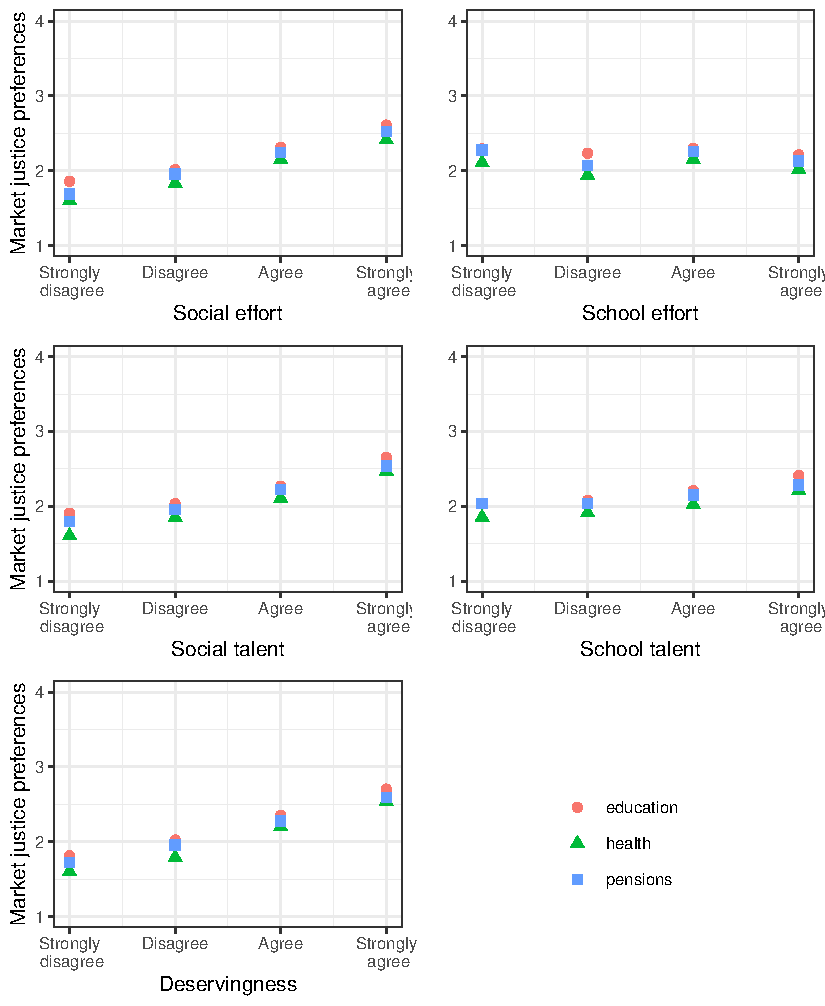
\includegraphics{paper_files/figure-pdf/fig-bivariate-1.pdf}

}

\caption{\label{fig-bivariate}Market justice preferences in education,
health and pensions by social and school meritocracy}

\end{figure}%

\subsection{Multivariate}\label{multivariate}

This section presents the results of the multilevel models. We begin by
showing the results of the cumulative link mixed models in
Table~\ref{tbl-ordinal-reg} for the ordinal dependent variables of
justice in health, pensions, and education separately in order to
compare the effect of the predictors. Then, we present the results of
the linear mixed-effects models for the average index of preference for
market justice in Table~\ref{tbl-lineal-reg}\footnote{The table shows
  the effects of individual and contextual-level independent variables
  related to our hypotheses; however, the models also incorporate the
  control variables for each of the three dependent variables separately
  and for the average index (complete models are available in the
  \hyperref[appendix]{Supplementary Material}).}.

For the health item, the intraclass correlation (ICC) obtained for the
null model (not shown) indicates that 5\% of the total variance of this
item is associated with specific characteristics of the schools, while
it is 3\% for the pensions item and 4\% for the education item
\citep[ICC based on][p.15]{hox_multilevel_2010}. For the average index
of market justice preferences, the ICC reaches 4\%, indicating that
overall, only a small percentage of the total variance in students'
market justice preferences is associated with school characteristics,
thus limiting the possibility of finding effects at this second level of
analysis.

\begin{table}

\caption{\label{tbl-ordinal-reg}Cumulative link multilevel models of
differential acces justificacion of health, pensions, and education}

\centering{

\begin{center}
\scalebox{0.8}{
\begin{threeparttable}
\begin{tabular}{l c c c c c c}
\toprule
 & \multicolumn{2}{c}{Health} & \multicolumn{2}{c}{Pensions} & \multicolumn{2}{c}{Education} \\
\cmidrule(lr){2-3} \cmidrule(lr){4-5} \cmidrule(lr){6-7}
 & Model 1 & Model 2 & Model 1 & Model 2 & Model 1 & Model 2 \\
\midrule
School talent                             & $0.23^{***}$  & $0.22^{***}$  & $0.17^{***}$  & $0.16^{***}$  & $0.25^{***}$  & $0.25^{***}$  \\
                                          & $(0.03)$      & $(0.03)$      & $(0.03)$      & $(0.03)$      & $(0.03)$      & $(0.03)$      \\
School effort                             & $-0.26^{***}$ & $-0.26^{***}$ & $-0.26^{***}$ & $-0.25^{***}$ & $-0.23^{***}$ & $-0.23^{***}$ \\
                                          & $(0.04)$      & $(0.04)$      & $(0.04)$      & $(0.04)$      & $(0.04)$      & $(0.04)$      \\
Social talent                             & $0.16^{***}$  & $0.16^{***}$  & $0.12^{**}$   & $0.13^{**}$   & $0.14^{**}$   & $0.15^{***}$  \\
                                          & $(0.05)$      & $(0.05)$      & $(0.04)$      & $(0.04)$      & $(0.04)$      & $(0.04)$      \\
Social effort                             & $0.11^{*}$    & $0.11^{*}$    & $0.27^{***}$  & $0.27^{***}$  & $0.15^{**}$   & $0.15^{**}$   \\
                                          & $(0.05)$      & $(0.05)$      & $(0.05)$      & $(0.05)$      & $(0.05)$      & $(0.05)$      \\
Deservingness                             & $0.52^{***}$  & $0.51^{***}$  & $0.38^{***}$  & $0.37^{***}$  & $0.44^{***}$  & $0.43^{***}$  \\
                                          & $(0.05)$      & $(0.05)$      & $(0.05)$      & $(0.05)$      & $(0.05)$      & $(0.05)$      \\
Parental education (Ref.= Non-university) &               &               &               &               &               &               \\
                                          &               &               &               &               &               &               \\
\quad University or posgraduate           & $0.05$        & $0.08$        & $0.14$        & $0.12$        & $0.09$        & $0.07$        \\
                                          & $(0.08)$      & $(0.08)$      & $(0.08)$      & $(0.08)$      & $(0.08)$      & $(0.08)$      \\
\quad Missing                             & $0.10$        & $0.11$        & $0.12^{*}$    & $0.11$        & $0.13^{*}$    & $0.12^{*}$    \\
                                          & $(0.06)$      & $(0.06)$      & $(0.06)$      & $(0.06)$      & $(0.06)$      & $(0.06)$      \\
More than 25 books (Ref.= Less than 25)   & $-0.16^{**}$  & $-0.13^{*}$   & $-0.13^{*}$   & $-0.13^{*}$   & $-0.07$       & $-0.07$       \\
                                          & $(0.06)$      & $(0.06)$      & $(0.06)$      & $(0.06)$      & $(0.06)$      & $(0.06)$      \\
Socioeconomic level (Ref.= Low)           &               &               &               &               &               &               \\
                                          &               &               &               &               &               &               \\
\quad SES Medium                          &               & $0.08$        &               & $0.02$        &               & $0.08$        \\
                                          &               & $(0.10)$      &               & $(0.10)$      &               & $(0.10)$      \\
\quad SES High                            &               & $0.71^{*}$    &               & $0.72^{**}$   &               & $0.93^{***}$  \\
                                          &               & $(0.28)$      &               & $(0.26)$      &               & $(0.28)$      \\
Achievement score (Ref.= Low)             &               &               &               &               &               &               \\
                                          &               &               &               &               &               &               \\
\quad Simce Medium                        &               & $-0.29^{***}$ &               & $-0.19^{*}$   &               & $-0.16^{*}$   \\
                                          &               & $(0.08)$      &               & $(0.08)$      &               & $(0.08)$      \\
\quad Simce High                          &               & $-0.56^{***}$ &               & $-0.53^{***}$ &               & $-0.46^{***}$ \\
                                          &               & $(0.10)$      &               & $(0.09)$      &               & $(0.10)$      \\
\midrule
Controls                                  & Yes           & Yes           & Yes           & Yes           & Yes           & Yes           \\
BIC                                       & $12747.58$    & $12761.47$    & $13103.81$    & $13112.87$    & $13329.33$    & $13352.18$    \\
Num.obs                                   & $5144$        & $5144$        & $5177$        & $5177$        & $5159$        & $5159$        \\
Num. groups: Schools                      & $231$         & $231$         & $232$         & $232$         & $231$         & $231$         \\
Var: Schools (Intercept)                  & $0.11$        & $0.05$        & $0.09$        & $0.04$        & $0.10$        & $0.05$        \\
\bottomrule
\end{tabular}
\begin{tablenotes}[flushleft]
\scriptsize{\item Note: Cells contain regression coefficients with standard errors in parentheses. Control variables are included. $^{***}p<0.001$; $^{**}p<0.01$; $^{*}p<0.05$ \\ \item Source: own elaboration based on First Study of Civic Education 2017.}
\end{tablenotes}
\end{threeparttable}
}
\caption{}
\label{table:coefficients}
\end{center}

}

\end{table}%

Model 1 in Table~\ref{tbl-ordinal-reg} for the three dependent variables
of justice in differential access to health, pensions, and education
demonstrates a similar trend regarding the effect of the perception of
meritocracy on these items, with all effects being statistically
significant (\emph{p} \textless{} 0.05). Regarding the variables of
social meritocracy, the three variables---talent, effort, and
deservingness---show that as these increase, the justification for
differentiated access to pensions, education, and health also increases.
In the context of school meritocracy, the effects are mixed: as
perceived school talent increases, the justification for differentiated
access to these services increases; conversely, as perceived school
effort increases, the justification decreases, holding all other
variables constant.

Additionally, Model 1 examines family status through parents'
educational level and the number of books at home. For health, pensions,
and education, a negative but statistically non-significant association
with parents' education is observed. However, having more than 25 books
at home shows a negative and statistically significant effect on market
justice in health and pensions, suggesting less justification for
differentiated access compared to those with fewer books.

Model 2 in Table~\ref{tbl-ordinal-reg} incorporates school-level
variables. The results show that high socioeconomic level schools show
greater preferences for market justice in health, pensions, and
education compared to low socioeconomic level schools, with
statistically significant results (\emph{p} \textless{} 0.05). Moreover,
and contrary to our hypothesis, schools with higher academic performance
show negative and statistically significant effects across the three
items.

\begin{table}

\caption{\label{tbl-lineal-reg}Linear mixed-effects models for
meritocracy perception and market justice preferences}

\centering{

\begin{center}
\scalebox{0.85}{
\begin{threeparttable}
\begin{tabular}{l c c c c}
\toprule
 & Model 1 & Model 2 & Model 3 & Model 4 \\
\midrule
Constant                                  & $1.31^{***}$  & $1.30^{***}$  & $1.36^{***}$  & $1.39^{***}$  \\
                                          & $(0.09)$      & $(0.10)$      & $(0.10)$      & $(0.10)$      \\
School talent                             & $0.11^{***}$  & $0.11^{***}$  & $0.10^{***}$  & $0.10^{***}$  \\
                                          & $(0.01)$      & $(0.01)$      & $(0.01)$      & $(0.01)$      \\
School effort                             & $-0.12^{***}$ & $-0.12^{***}$ & $-0.12^{***}$ & $-0.12^{***}$ \\
                                          & $(0.02)$      & $(0.02)$      & $(0.02)$      & $(0.02)$      \\
Social talent                             & $0.07^{***}$  & $0.07^{***}$  & $0.07^{***}$  & $0.07^{***}$  \\
                                          & $(0.02)$      & $(0.02)$      & $(0.02)$      & $(0.02)$      \\
Social effort                             & $0.08^{***}$  & $0.08^{***}$  & $0.08^{***}$  & $0.08^{***}$  \\
                                          & $(0.02)$      & $(0.02)$      & $(0.02)$      & $(0.02)$      \\
Deservingness                             & $0.20^{***}$  & $0.20^{***}$  & $0.20^{***}$  & $0.20^{***}$  \\
                                          & $(0.02)$      & $(0.02)$      & $(0.02)$      & $(0.02)$      \\
Parental education (Ref.= Non-university) &               &               &               &               \\
                                          &               &               &               &               \\
\quad University or posgraduate           &               & $0.05$        & $0.05$        & $0.05$        \\
                                          &               & $(0.03)$      & $(0.04)$      & $(0.04)$      \\
\quad Missing                             &               & $0.06^{*}$    & $0.06^{*}$    & $0.06^{*}$    \\
                                          &               & $(0.03)$      & $(0.03)$      & $(0.03)$      \\
More than 25 books (Ref.= Less than 25)   &               & $-0.05$       & $-0.05$       & $-0.04$       \\
                                          &               & $(0.03)$      & $(0.03)$      & $(0.03)$      \\
Socioeconomic level (Ref.= Low)           &               &               &               &               \\
                                          &               &               &               &               \\
\quad SES Medium                          &               &               & $-0.01$       & $0.01$        \\
                                          &               &               & $(0.05)$      & $(0.05)$      \\
\quad SES High                            &               &               & $0.31^{*}$    & $0.37^{**}$   \\
                                          &               &               & $(0.14)$      & $(0.13)$      \\
Achievement score (Ref.= Low)             &               &               &               &               \\
                                          &               &               &               &               \\
\quad Simce Medium                        &               &               &               & $-0.11^{**}$  \\
                                          &               &               &               & $(0.04)$      \\
\quad Simce High                          &               &               &               & $-0.26^{***}$ \\
                                          &               &               &               & $(0.04)$      \\
\midrule
Controls                                  & Yes           & Yes           & Yes           & Yes           \\
Deviance                                  & $12368.01$    & $12359.40$    & $12344.10$    & $12310.90$    \\
Deviance Test (p)                         & $0.00$        & $0.00$        & $0.00$        & $0.00$        \\
BIC                                       & $12517.46$    & $12550.41$    & $12595.11$    & $12589.48$    \\
Num.obs                                   & $5047$        & $5047$        & $5047$        & $5047$        \\
Num. groups: Schools                      & $231$         & $231$         & $231$         & $231$         \\
Var: Schools (Intercept)                  & $0.02$        & $0.02$        & $0.02$        & $0.01$        \\
Var: Residual                             & $0.66$        & $0.66$        & $0.67$        & $0.66$        \\
\bottomrule
\end{tabular}
\begin{tablenotes}[flushleft]
\scriptsize{\item Note: Cells contain regression coefficients with standard errors in parentheses. Control variables are included. $^{***}p<0.001$; $^{**}p<0.01$; $^{*}p<0.05$ \\ \item Source: own elaboration based on First Study of Civic Education 2017.}
\end{tablenotes}
\end{threeparttable}
}
\caption{}
\label{table:coefficients}
\end{center}

}

\end{table}%

Table~\ref{tbl-lineal-reg} presents the results of linear mixed-effects
models for the market justice preference index. Model 1 shows that
higher perceived societal meritocracy, through effort, talent, and
deservingness, is positively and significantly associated with market
justice preferences. School meritocracy perceptions yield mixed effects:
perceived talent increases market justice preference, while perceived
effort decreases it, both statistically significant (\emph{p}
\textless{} 0.001). Model 2 includes family status, finding no
statistically significant effects from parents' education or the number
of books at home. Regarding school characteristics, Models 3 and 4
introduce socioeconomic level and academic performance. The results of
Model 3 suggest a statistically significant relationship between school
socioeconomic levels and market justice preferences, specifically those
schools with high socioeconomic levels (\(\beta\) = 0.37) compared to
low socioeconomic levels. However, Model 4 indicates that schools with
medium (\(\beta\) = -0.11) and high (\(\beta\) = -0.26) academic
performance present lower market justice preferences compared to
low-performing schools, with these effects being statistically
significant when controlling for other variables.

\begin{table}

\caption{\label{tbl-interact}Interactions effects}

\centering{

\resizebox{\linewidth}{!}{
\begin{tabu} to \linewidth {>{\raggedright\arraybackslash}p{4cm}>{\centering\arraybackslash}p{1.5cm}>{\centering\arraybackslash}p{1.5cm}>{\centering\arraybackslash}p{1.5cm}>{\centering\arraybackslash}p{1.5cm}>{\centering\arraybackslash}p{1.5cm}}
\toprule
\multicolumn{1}{c}{\textbf{ }} & \multicolumn{5}{c}{\textbf{Market Justice Preferences}} \\
\cmidrule(l{3pt}r{3pt}){2-6}
Variable & School talent & School effort & Social talent & Social effort & Deservingness\\
\midrule
\textbf{University or Postgraduate} & -0.034 & -0.012 & -0.073. & -0.079* & -0.118**\\
\cmidrule{1-6}
\textbf{More than 25 books} & -0.015 & -0.046 & -0.029 & -0.081** & -0.035\\
\cmidrule{1-6}
\textbf{School SES high} & 0.004 & 0.001 & -0.057. & -0.063* & -0.08**\\
\cmidrule{1-6}
\textbf{Simce Medium} & 0.001 & 0.032 & -0.037 & -0.041 & -0.082*\\
\cmidrule{1-6}
\textbf{Simce High} & -0.016 & 0.008 & -0.043 & -0.063. & -0.087*\\
\bottomrule
\multicolumn{6}{l}{\textsuperscript{} Note: ***p < 0.001, **p < 0.01, *p < 0.05. Source: own elaboration based on First Study of Civic}\\
\multicolumn{6}{l}{Education 2017.}\\
\end{tabu}}

}

\end{table}%

Table~\ref{tbl-interact} displays the interaction terms related to our
hypotheses. The results suggest that students' family background
moderates the relationship between their meritocratic perceptions and
their justification of market allocation in social services.
Specifically, the relationship between social effort and market justice
preferences is less positive for students whose parents have university
or postgraduate education. Lower-status students (measured by parental
education) prefer more market justice when they strongly adhere to
meritocratic perceptions of deservingness. A similar moderating effect
is seen with family cultural capital: the relationship between effort
and market justice preferences is less positive for students with more
than 25 books at home.

At the school level, we observe that school status and students'
meritocratic beliefs moderate their preferences for market justice.
High-status schools show less preference for market justice when their
students, on average, have a greater perception of meritocracy, as
measured by effort, deservingness, and talent. Conversely, low-achieving
schools prefer more market justice when their students have stronger
meritocratic beliefs. Figure~\ref{fig-interaction} illustrates this
moderating effect of school achievement on the relationship between
deservingness and market justice. No moderating effects were observed at
the school level for students' meritocratic beliefs regarding effort or
talent in achieving good grades.

\begin{figure}

\centering{

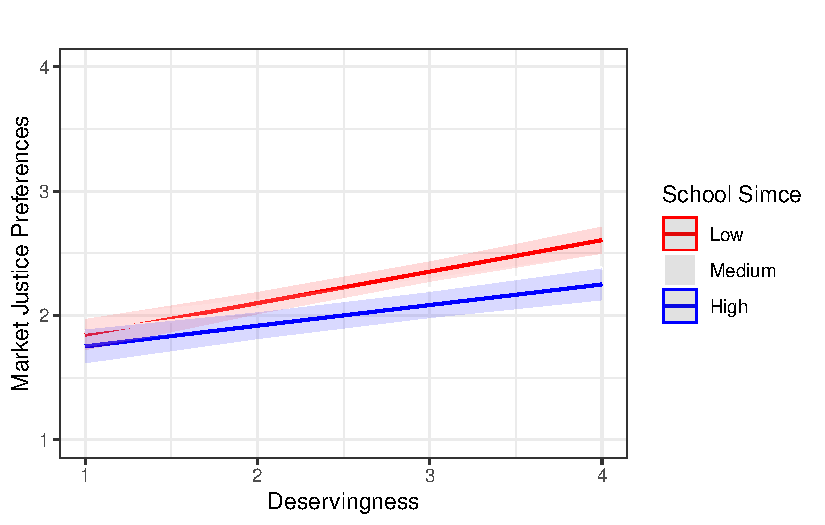
\includegraphics{paper_files/figure-pdf/fig-interaction-1.pdf}

}

\caption{\label{fig-interaction}Interaction between deservingness and
justification of inequality by school SIMCE achievement}

\end{figure}%

\section{Discussion}\label{discussion}

The previous analyses aimed to explore the relationship between
perceptions of meritocracy and preferences for market justice among
students in Chilean society. Several models estimated how students'
beliefs about the rewards for talent and effort in both societal and
school contexts influence their attitudes toward access to social
services like health, education, and pensions based on pay capacity.
Additionally, the models examined the impact of students' socioeconomic
status and school achievement on these preferences, assessing whether
perceptions of meritocracy moderate these effects. The findings offer
insights into the complex interplay between meritocratic beliefs,
socioeconomic factors, and attitudes toward market justice criteria.

Hypothesis \(H_{1a}\) posited that students who perceive greater
meritocracy in society would show stronger preferences for market
justice. The results support this hypothesis, indicating a positive
relationship between the perception that talent and effort are rewarded
in society and the preferences for market justice in access to services
such as health, education, and pensions. This finding aligns with
previous research suggesting that individuals who believe in a
meritocratic system are more likely to justify social inequalities
\citep{batruch_belief_2022, wiederkehr_belief_2015}. It is noteworthy
that among the items measuring meritocratic perception, consistently the
one about deservingness shows a larger effect when compared to the ones
about talent and effort. Although the three items correlate, there is
something distinctive about deservingness that probably encompasses
other aspects beyond meritocracy, an aspect to which we will come back
in the conclusions. Moving now to hypothesis \(H_{1b}\), this is simply
a variation of 1a, replacing the perception of meritocracy at society by
the one at school. In this case we have only two items of meritocratic
perception - unfortunately deservingness was not measured at school
level - and the direction of the effects is not as straightforward as in
the case of societal meritocracy in \(H_{1a}\): positive for talent, but
negative for effort. Still, one of the limitation for the comparison
between perception of meritocracy and society is the difference of the
items' phrasing. Whereas for society the item refers to the extent to
which efforts are rewarded, at school is about the importance of effort,
whereby something that is important does not necessarily mean that it is
enough to be rewarded. Furthermore, the school-effort item is the one
with the lowest variation among all meritocratic items (more than 95\%
agree or strongly agree), and with the lowest effect size.

Hypothesis \(H_2\) and hypothesis \(H_3\) propose that socioeconomic
status could influence students' preferences, but the results show
different patterns. On the one hand, \(H_2\) proposed that students from
higher socioeconomic status families would show stronger preferences for
market justice, which is not supported by the results. Although students
from families with higher educational levels and more economic resources
tend to prefer less market justice, this relationship is not
statistically significant. This might be due to the influence of other
contextual and cultural factors that modulate attitudes toward market
justice \citep{kohn_social_1963, kohn_class_1969, almas_fairness_2017}.
Notably, socioeconomic status measured by parental educational level and
the number of books at home do not explain variations in market justice
preferences, suggesting that other variables, such as market justice
preferences of parents, could play an essential role in the attitudinal
socialization process. On the other hand, Hypothesis \(H_3\) held that
students from schools with higher socioeconomic status would show
stronger preferences for market justice. The results confirm this
hypothesis since students from high-status schools tend to prefer more
market justice, compared to low-status schools. This finding, in line
with the existing literature
\citep{jonsson_institutional_2015, jost_attitudinal_2000}, does allow us
to affirm the hypothesis about the role of the school environment,
particularly socioeconomic segregation, in influencing attitudes towards
market justice and the acceptance of inequalities. A possible
explanation is the role of the context at the school level, which could
have a more relevant role than the family socioeconomic status, since
the highly stratified nature of the Chilean education system reinforces
socioeconomic divisions and socializes students into different normative
frameworks.

Hypothesis \(H_4\) held that students from schools with higher school
achievement would show stronger preferences for market justice,
following the argument that such schools could foster meritocratic
attitudes by showing a larger promotion of talent and effort in order to
get better results. Nevertheless, the results show quite the opposite:
schools with better academic results (as measured by a national
standardized test) show in average less preferences for market justice.
This finding is one of the most strongest and consistent throughout the
models and it is relevant given the centrality of school performance in
educational institutions. One possible explanation of this link is that
students in high-achieving schools may be more exposed to discussions
and a deeper understanding of inequality and social justice, leading to
a critical perspective toward the weight of market mechanisms in the
access to social services.

Hypotheses \(H_5\) and \(H_6\) proposed that socioeconomic status would
moderate the effect of meritocratic perceptions on market justice
preferences. Hypothesis \(H_5\) refers to family socioeconomic status,
whereby the results show a negative interaction with two of the three
perceptual variables at the societal level. This means that the positive
impact of the perception of social meritocracy on market justice
preferences had a lower effect on students with parents with higher
education and also on those with more books at home. Something similar
occurs with hypothesis \(H_6\), where now school-level status moderates
the effect of meritocracy variables, which in multilevel framework is
referred as to cross-level interaction. The negative interaction in this
context means that in schools of low socioeconomic levels, the positive
effect of the social meritocracy variables on market justice preferences
is stronger. These relations indicate that, although those who perceive
society as meritocratic have greater preferences towards market justice,
this influence is lower among those with a higher socioeconomic level.
This finding highlights the complex interaction between socioeconomic
status, school context, meritocratic beliefs, and preferences toward
market justice. The moderating role of meritocratic perceptions suggests
that students' views on social justice are shaped by their socioeconomic
background and beliefs about how society rewards effort and talent. This
underlines the importance of addressing structural inequalities and
individual beliefs in educational and social policies.

Hypothesis \(H7\) posited that the academic performance of schools could
moderate the effect of meritocratic perceptions on preferences for
market justice. This hypothesis is based on the argument that the level
of academic performance in schools entails a differentiated promotion of
meritocratic perceptions to achieve better results, which would, in
turn, reinforce or diminish preferences for market justice. The results
of the interactions between levels suggest that, indeed, in
higher-performing schools, the effect of meritocratic perceptions on the
justification of service provision based on market principles is weaker
compared to lower-performing schools. Similarly to the effect of
academic performance in \(H4\), a possible explanation for this
moderation is that students in high-performing schools may be more
exposed to knowledge about the effects of inequality and social justice.
This exposure translates into an enlightening effect of education on
inequality, which can mitigate the impact of meritocracy on market
justice preferences.

\section{Conclusion}\label{conclusion}

Our research aimed to examine the relationship between the perception of
meritocracy and the justification of market justice preferences among
eighth-grade students in Chile. From our knowledge this is the first
study addressing market justice preferences at school level, finding
that students exhibit large preferences for market justice (about one
third agree or strongly agree with them), a share that is quite larger
when compared with evidence in adult population. Perception of
meritocracy is also high, particularly when it comes to the reward of
effort, with an striking eighty six percent of agreement. Regarding
these descriptive indicators, a a first message coming from this study
is that there is something particular in school-age when it comes to
perceptions and preferences about inequality. This can relate to
development aspects
\citep[\citet{rizzo_children_2020}]{kim_socioeconomic_2020} but it could
be something specific to the Chilean case, which requires further
comparative as well as longitudinal research in the area. In any case,
teaching about the origins and characteristics of social inequality is
not part of the chilean school curriculum, calling for a more dedicated
consideration of these topics in areas such as citizensip education as
well as in history and social science education.

The core of this paper was the association between meritocratic
perceptions and preferences for market justice. In general, we find that
those who perceive that effort and talent/intelligence are rewarded, are
more willing to agree with that richer individuals can have better
health, education, and pensions. This is not the first time that
meritocratic perceptions (and also beliefs) have been related with the
legitimation of social inequalities
\citep{mijs_paradox_2019, darnon_where_2018}, but the consideration of
school level population as well as market justice preferences allows
adding evidence regarding the role of meritocracy regarding inequality
beliefs: legitimation of market criteria in social services seems to
begin at school age, and what students think of meritocracy is linked to
it. Although there are still several open questions, as for instance
differences between meritocratic perceptions in school and in the
society at large, this raises up the relevance of what is done (or not)
in schools in order to challenge the meritocratic ideals.

The consideration of the school context opened some caveats in this
research. We found contrary evidence for the association between status,
school performance, and market justice preferences: high status and high
achievement at the school level are associated with less market justice
preferences. This is opposed to the rational-interest argument that
suggests that those doing better - both economically and academically-
would demand less redistribution \citep[\citet{runst_does_2018},
\citet{bullock_education_2021}]{gonthier_parallel_2017} and therefore
are expected to challenge market mechanisms. A possible explanation is
that education contributes to forming a critical view of markets in
redistribution, nevertheless, further research in this area is needed to
assert the specific mechanisms that might be playing a role. All in all,
from this study we know that school contexts are not trivial in this
regard, calling for larger attention to school-age research on the
formation of inequality preferences and beliefs.

%\authorcontributions{For research articles with several authors, a short paragraph specifying their individual contributions must be provided. The following statements should be used ``Conceptualization, X.X. and Y.Y.; methodology, X.X.; software, X.X.; validation, X.X., Y.Y. and Z.Z.; formal analysis, X.X.; investigation, X.X.; resources, X.X.; data curation, X.X.; writing---original draft preparation, X.X.; writing---review and editing, X.X.; visualization, X.X.; supervision, X.X.; project administration, X.X.; funding acquisition, Y.Y. All authors have read and agreed to the published version of the manuscript.'', please turn to the  \href{http://img.mdpi.org/data/contributor-role-instruction.pdf}{CRediT taxonomy} for the term explanation. Authorship must be limited to those who have contributed substantially to the work~reported.}

}


%\funding{Please add: ``This research received no external funding'' or ``This research was funded by NAME OF FUNDER grant number XXX.'' and  and ``The APC was funded by XXX''. Check carefully that the details given are accurate and use the standard spelling of funding agency names at \url{https://search.crossref.org/funding}, any errors may affect your future funding.}



%\institutionalreview{In this section, you should add the Institutional Review Board Statement and approval number, if relevant to your study. You might choose to exclude this statement if the study did not require ethical approval. Please note that the Editorial Office might ask you for further information. Please add “The study was conducted in accordance with the Declaration of Helsinki, and approved by the Institutional Review Board (or Ethics Committee) of NAME OF INSTITUTE (protocol code XXX and date of approval).” for studies involving humans. OR “The animal study protocol was approved by the Institutional Review Board (or Ethics Committee) of NAME OF INSTITUTE (protocol code XXX and date of approval).” for studies involving animals. OR “Ethical review and approval were waived for this study due to REASON (please provide a detailed justification).” OR “Not applicable” for studies not involving humans or animals.}



%\informedconsent{Any research article describing a study involving humans should contain this statement. Please add ``Informed consent was obtained from all subjects involved in the study.'' OR ``Patient consent was waived due to REASON (please provide a detailed justification).'' OR ``Not applicable'' for studies not involving humans. You might also choose to exclude this statement if the study did not involve humans. Written informed consent for publication must be obtained from participating patients who can be identified (including by the patients themselves). Please state ``Written informed consent has been obtained from the patient(s) to publish this paper'' if applicable.}



%\dataavailability{We encourage all authors of articles published in MDPI journals to share their research data. In this section, please provide details regarding where data supporting reported results can be found, including links to publicly archived datasets analyzed or generated during the study. Where no new data were created, or where data is unavailable due to privacy or ethical restrictions, a statement is still required. Suggested Data Availability Statements are available in section ``MDPI Research Data Policies'' at \url{https://www.mdpi.com/ethics}.} 



% Only for journal Nursing Reports
%\publicinvolvement{Please describe how the public (patients, consumers, carers) were involved in the research. Consider reporting against the GRIPP2 (Guidance for Reporting Involvement of Patients and the Public) checklist. If the public were not involved in any aspect of the research add: ``No public involvement in any aspect of this research''.}

% Only for journal Nursing Reports
%\guidelinesstandards{Please add a statement indicating which reporting guideline was used when drafting the report. For example, ``This manuscript was drafted against the XXX (the full name of reporting guidelines and citation) for XXX (type of research) research''. A complete list of reporting guidelines can be accessed via the equator network: \url{https://www.equator-network.org/}.}

%\acknowledgments{In this section you can acknowledge any support given which is not covered by the author contribution or funding sections. This may include administrative and technical support, or donations in kind (e.g., materials used for experiments).}



%\conflictsofinterest{Declare conflicts of interest or state ``The authors declare no conflicts of interest.'' Authors must identify and declare any personal circumstances or interest that may be perceived as inappropriately influencing the representation or interpretation of reported research results. Any role of the funders in the design of the study; in the collection, analyses or interpretation of data; in the writing of the manuscript; or in the decision to publish the results must be declared in this section. If there is no role, please state ``The funders had no role in the design of the study; in the collection, analyses, or interpretation of data; in the writing of the manuscript; or in the decision to publish the results''.} 



\begin{adjustwidth}{-\extralength}{0cm}
%\printendnotes[custom] % Un-comment to print a list of endnotes

\reftitle{References}

  \bibliography{input/bib/just-ineq-merit.bib}


\PublishersNote{}
\end{adjustwidth}\end{document}
